\documentclass{article}
\usepackage[paperwidth=18.25cm,paperheight=7.45cm,margin=0cm]{geometry}
\usepackage{tikz}
\usepackage{xcolor}
\pagestyle{empty}

\definecolor{a100green}{HTML}{70AD47}
\definecolor{qdareorange}{HTML}{F4A340}
\definecolor{gridgray}{HTML}{D9D9D9}
\definecolor{axisgray}{HTML}{595959}
\definecolor{gainred}{HTML}{C00000}

\begin{document}
\noindent
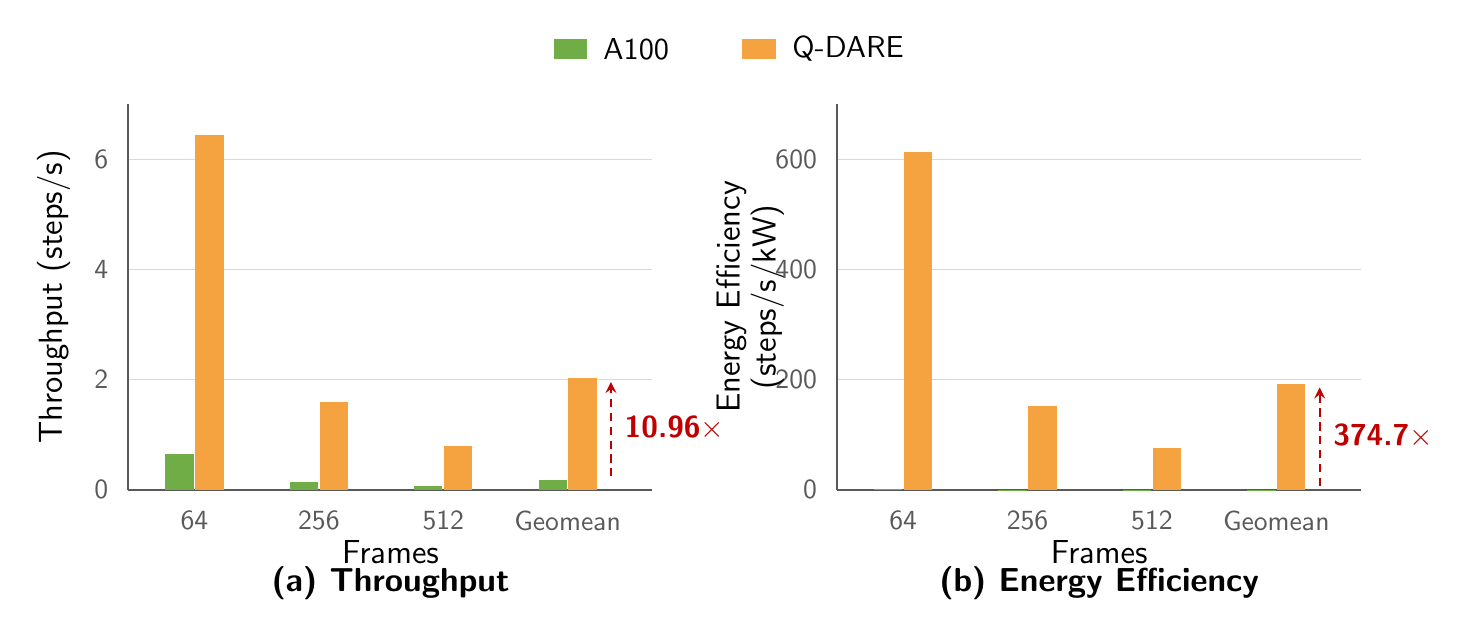
\begin{tikzpicture}[x=1cm,y=1cm]
  \tikzset{
    tick/.style={font=\sffamily\fontsize{10}{11}\selectfont,text=axisgray},
    label/.style={font=\sffamily\fontsize{12}{13}\selectfont,text=black},
    title/.style={font=\sffamily\bfseries\fontsize{12}{13}\selectfont,text=black},
    legend/.style={font=\sffamily\fontsize{11}{12}\selectfont,text=black},
    gain/.style={font=\sffamily\bfseries\fontsize{11}{12}\selectfont,text=gainred},
  }

  % Shared legend.
  \fill[a100green] (6.65,6.82) rectangle +(0.42,0.25);
  \node[legend,anchor=west] at (7.16,6.945) {A100};
  \fill[qdareorange] (9.05,6.82) rectangle +(0.42,0.25);
  \node[legend,anchor=west] at (9.56,6.945) {Q-DARE};

  % (a) Throughput, plot origin=(1.25,1.35), size=6.65 x 4.9, ymax=7.
  \foreach \value/\yy in {0/1.35,2/2.75,4/4.15,6/5.55} {
    \draw[gridgray,line width=0.35pt] (1.25,\yy) -- (7.90,\yy);
    \node[tick,anchor=east] at (1.12,\yy) {\value};
  }
  \draw[axisgray,line width=0.65pt] (1.25,1.35) -- (7.90,1.35);
  \draw[axisgray,line width=0.65pt] (1.25,1.35) -- (1.25,6.25);
  \node[label,rotate=90] at (0.30,3.80) {Throughput (steps/s)};

  % A100 and Q-DARE bars: 64, 256, 512, geomean.
  \fill[a100green]   (1.72,1.35) rectangle (2.08,1.800);
  \fill[qdareorange] (2.10,1.35) rectangle (2.46,5.862);
  \fill[a100green]   (3.30,1.35) rectangle (3.66,1.452);
  \fill[qdareorange] (3.68,1.35) rectangle (4.04,2.472);
  \fill[a100green]   (4.88,1.35) rectangle (5.24,1.397);
  \fill[qdareorange] (5.26,1.35) rectangle (5.62,1.910);
  \fill[a100green]   (6.46,1.35) rectangle (6.82,1.479);
  \fill[qdareorange] (6.84,1.35) rectangle (7.20,2.765);

  \foreach \xx/\name in {2.09/64,3.67/256,5.25/512,6.83/Geomean} {
    \node[tick,anchor=north] at (\xx,1.20) {\name};
  }
  \draw[gainred,densely dashed,->,>=stealth,line width=0.75pt]
    (7.38,1.52) -- (7.38,2.72);
  \node[gain,anchor=west] at (7.43,2.13) {10.96$\times$};
  \node[label] at (4.58,0.56) {Frames};
  \node[title] at (4.58,0.16) {(a) Throughput};

  % (b) Energy efficiency, origin=(10.25,1.35), size=6.65 x 4.9, ymax=700.
  \foreach \value/\yy in {0/1.35,200/2.75,400/4.15,600/5.55} {
    \draw[gridgray,line width=0.35pt] (10.25,\yy) -- (16.90,\yy);
    \node[tick,anchor=east] at (10.12,\yy) {\value};
  }
  \draw[axisgray,line width=0.65pt] (10.25,1.35) -- (16.90,1.35);
  \draw[axisgray,line width=0.65pt] (10.25,1.35) -- (10.25,6.25);
  \node[label,align=center,rotate=90] at (9.15,3.80)
    {Energy Efficiency\\(steps/s/kW)};

  \fill[a100green]   (10.72,1.35) rectangle (11.08,1.362);
  \fill[qdareorange] (11.10,1.35) rectangle (11.46,5.644);
  \fill[a100green]   (12.30,1.35) rectangle (12.66,1.353);
  \fill[qdareorange] (12.68,1.35) rectangle (13.04,2.418);
  \fill[a100green]   (13.88,1.35) rectangle (14.24,1.351);
  \fill[qdareorange] (14.26,1.35) rectangle (14.62,1.883);
  \fill[a100green]   (15.46,1.35) rectangle (15.82,1.354);
  \fill[qdareorange] (15.84,1.35) rectangle (16.20,2.697);

  \foreach \xx/\name in {11.09/64,12.67/256,14.25/512,15.83/Geomean} {
    \node[tick,anchor=north] at (\xx,1.20) {\name};
  }
  \draw[gainred,densely dashed,->,>=stealth,line width=0.75pt]
    (16.38,1.40) -- (16.38,2.65);
  \node[gain,anchor=west] at (16.43,2.03) {374.7$\times$};
  \node[label] at (13.58,0.56) {Frames};
  \node[title] at (13.58,0.16) {(b) Energy Efficiency};
\end{tikzpicture}
\end{document}
